\documentclass[a4paper,11pt,bahasa]{extarticle}
\usepackage[a4paper]{geometry}
\geometry{verbose,tmargin=2cm,bmargin=2cm,lmargin=2cm,rmargin=2cm}

\usepackage{fontspec}
\setmonofont{FreeMono}

\setlength{\parindent}{0cm}
\setlength{\parskip}{0.5em}

\usepackage{textcomp}

\usepackage{hyperref}
\usepackage{url}
\usepackage{xcolor}

\usepackage{minted}
\newminted{python}{breaklines,fontsize=\footnotesize}
\newminted{text}{breaklines,fontsize=\footnotesize}

\definecolor{mintedbg}{rgb}{0.95,0.95,0.95}
\usepackage{mdframed}

%\BeforeBeginEnvironment{minted}{\begin{mdframed}[backgroundcolor=mintedbg]}
%\AfterEndEnvironment{minted}{\end{mdframed}}

\usepackage{babel}

\title{
MI3103 \\
Pengenalan Protokol HTTP}
\author{Fadjar Fathurrahman}
\date{2018}

\begin{document}
\maketitle

\tableofcontents

\section{Overview}

HTTP adalah singkatan dari Hypertext Transfer Protocol. HTTP merupakan protokol
jaringan tingkat aplikasi untuk sistem informasi terdistribusi, kolaboratif,
dan hypermedia. Protokol ini merupakan fondasi bagi komunikasi data untuk
World Wide Web (W3, internet) sejak tahun 1990. HTTP juga
dapat digunakan untuk keperluan selain World Wide Web.
HTTP dispesifikasikan dalam RFC-2616, yang mendefinisikan protokol yang
dikenal sekarang sebagai HTTP/1.1, yang merupakan revisi dari HTTP awal
(HTTP/1.0). Perbedaan penting antara HTTP/1.1 dan HTTP/1.0 adalah HTTP/1.0
menggunakan koneksi baru untuk tiap pertukaran permintaan (\textit{request})
dan respon (\textit{response}), sedangkan pada HTTP/1.1 satu koneksi
dapat digunakan untuk pertukaran lebih dari satu
\textit{request}/\textit{response}.

HTTP adalah protokol komunikasi yang berbasis TCP/IP, yang digunakan
untuk mengirimkan data seperti file HTML, CSS, Javascript, gambar, dan
sebagainya melalui Web.
Port default untuk protokol TCP adalah 80, meskipun port lain juga dapat
digunakan.
HTTP menyediakan cara standard bagi komputer untuk berkomunikasi
satu dengan yang lainnya.
HTTP menspesifikasikan bagaimanan data permintaan
dari klien dibangung dan dikirimkan ke server, serta bagaimana
server merespon permintaan tersebut.

Fitur dasar HTTP:
\begin{itemize}
\item Connectionless: Klien HTTP menginisiasi permintaan HTTP dan setelah itu klien
melepas koneksi dengan server dan menunggu respon dari server. Proses server
menerima permintaan dan membangun kembali koneksi dengan klien untuk
mengirimkan respon.
\item Media-independent: tipe data apapun dapat dikirimkan melalui HTTP asalkan
klien dan server mengetahui bagaimana cara menangani data tersebut.
\item Stateless: As mentioned above, HTTP is connectionless and it
is a direct result of HTTP being a stateless protocol.
The server and client are aware of each other only during a
current request. Afterwards, both of them forget about each other.
Due to this nature of the protocol, neither the client nor the
browser can retain information between different requests across the web pages.
\end{itemize}

HTTP/1.0 uses a new connection for each request/response exchange,
where as HTTP/1.1 connection may be used for one or more request/response exchanges.

Basic Architecture

The following diagram shows a very basic architecture of a web application and
depicts where HTTP sits:

HTTP Architecture

{\centering
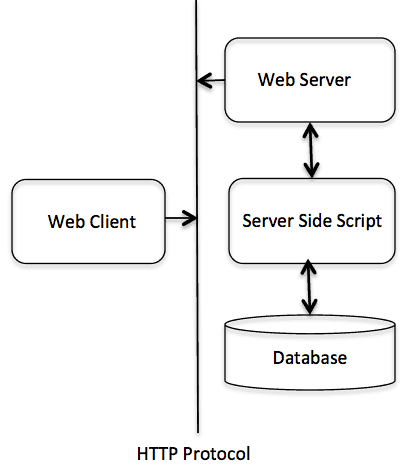
\includegraphics[scale=1.0]{images/cgiarch.png}
}

The HTTP protocol is a request/response protocol based on the client/server based architecture 
where web browsers, robots and search engines, etc. act like HTTP clients, and the Web server 
acts as a server.

Client

The HTTP client sends a request to the server in the form of a request method, URI, and protocol 
version, followed by a MIME-like message containing request modifiers, client information, and 
possible body content over a TCP/IP connection.

Server

The HTTP server responds with a status line, including the message's protocol version and a 
success or error code, followed by a MIME-like message containing server information, entity meta 
information, and possible entity-body content.

\section{HTTP parameters}

This chapter is going to list down few of the important HTTP Protocol Parameters
and their syntax the way they are used in the communication. For example, format
for date, format of URL, etc. This will help you in constructing your request and
response messages while writing HTTP client or server programs. You will see the
complete usage of these parameters in subsequent chapters while learning the message
structure for HTTP requests and responses.

\subsection{HTTP Version}

HTTP uses a \verb|<major>.<minor>| numbering scheme to indicate versions of the protocol.
The version of an HTTP message is indicated by an HTTP-Version field in the first line.
Here is the general syntax of specifying HTTP version number:
\begin{textcode}
HTTP-Version   = "HTTP" "/" 1*DIGIT "." 1*DIGIT
\end{textcode}
Example
\begin{textcode}
HTTP/1.0
\end{textcode}
or
\begin{textcode}
HTTP/1.1
\end{textcode}

\subsection{Uniform Resource Identifiers}

Uniform Resource Identifiers (URI) are simply formatted, case-insensitive string containing name, 
location, etc. to identify a resource, for example, a website, a web service, etc. A general syntax of 
URI used for HTTP is as follows:

\begin{textcode}
URI = "http:" "//" host [ ":" port ] [ abs_path [ "?" query ]]
\end{textcode}

Here if the port is empty or not given, port 80 is assumed for HTTP and an empty
\verb|abs_path| is equivalent 
to an \verb|abs_path| of "/".
The characters other than those in the reserved and unsafe sets are equivalent to 
their \verb|""%" HEX HEX"| encoding.

Examples: the following three URIs are equivalent:
\begin{textcode}
http://abc.com:80/~smith/home.html
http://ABC.com/%7Esmith/home.html
http://ABC.com:/%7esmith/home.html
\end{textcode}

\subsection{Date/Time Formats}

All HTTP date/time stamps MUST be represented in Greenwich Mean Time (GMT), without exception. HTTP 
applications are allowed to use any of the following three representations of date/time stamps:

\begin{textcode}
Sun, 06 Nov 1994 08:49:37 GMT  ; RFC 822, updated by RFC 1123
Sunday, 06-Nov-94 08:49:37 GMT ; RFC 850, obsoleted by RFC 1036
Sun Nov  6 08:49:37 1994       ; ANSI C's asctime() format
\end{textcode}

\subsection{Character Sets}

We use character sets to specify the character sets that the client prefers. Multiple
character sets can  be listed separated by commas. If a
value is not specified, the default is the US-ASCII.

Example: Following are the valid character sets:
\begin{itemize}
\item US-ASCII
\item ISO-8859-1
\item ISO-8859-7
\end{itemize}

\subsection{Content Encodings}

A content encoding value indicates that an encoding algorithm has been used to encode the
content before passing it over the network. Content coding are primarily used to allow a document to be 
compressed or otherwise usefully transformed without losing the identity.

All content-coding values are case-insensitive. HTTP/1.1 uses content-coding values in the 
Accept-Encoding and Content-Encoding header fields which we will see in the subsequent chapters.

Examples: The following are valid encoding schemes:
\begin{textcode}
Accept-encoding: gzip
Accept-encoding: compress
Accept-encoding: deflate
\end{textcode}

\subsection{Media Types}

HTTP uses Internet Media Types in the Content-Type and Accept header fields in order to
provide open and extensible data typing and type negotiation. All the Media-type values
are registered with the Internet Assigned Number Authority (IANA). The general syntax to
specify media type is as follows:
\begin{textcode}
media-type     = type "/" subtype *( ";" parameter )
\end{textcode}
The type, subtype, and parameter attribute names are case-insensitive. Example
\begin{textcode}
Accept: image/gif
\end{textcode}

\subsection{Language Tags}
HTTP uses language tags within the Accept-Language and Content-Language fields. A language tag is 
composed of one or more parts: a primary language tag and a possibly empty series of subtags:
\begin{textcode}
language-tag  = primary-tag *( "-" subtag )
\end{textcode}
White spaces are not allowed within the tag and all tags are case-insensitive.
Example tags include:
\begin{textcode}
en, en-US, en-cockney, i-cherokee, x-pig-latin
\end{textcode}
where any two-letter primary-tag is an ISO-639 language abbreviation and any two-letter initial subtag 
is an ISO-3166 country code.


\section{HTTP - Messages}

HTTP is based on the client-server architecture model and a stateless request/response protocol that 
operates by exchanging messages across a reliable TCP/IP connection.

An HTTP "client" is a program (Web browser or any other client) that establishes a connection to a 
server for the purpose of sending one or more HTTP request messages. An HTTP "server" is a program ( 
generally a web server like Apache Web Server or Internet Information Services IIS, etc. ) that accepts 
connections in order to serve HTTP requests by sending HTTP response messages.

HTTP makes use of the Uniform Resource Identifier (URI) to identify a given resource and to establish a 
connection. Once the connection is established, HTTP messages are passed in a format similar to that 
used by the Internet mail [RFC5322] and the Multipurpose Internet Mail Extensions (MIME) [RFC2045]. 
These messages include requests from client to server and responses from server to client which will 
have the following format:
\begin{textcode}
HTTP-message   = <Request> | <Response> ; HTTP/1.1 messages
\end{textcode}

HTTP requests and HTTP responses use a generic message format of RFC 822 for transferring the required 
data. This generic message format consists of the following four items.
\begin{textcode}
    A Start-line

    Zero or more header fields followed by CRLF

    An empty line (i.e., a line with nothing preceding the CRLF) 
    indicating the end of the header fields

    Optionally a message-body
\end{textcode}

In the following sections, we will explain each of the entities used in an HTTP message.

\subsection{Message Start-Line}

A start-line will have the following generic syntax:
\begin{textcode}
start-line = Request-Line | Status-Line
\end{textcode}

We will discuss Request-Line and Status-Line while discussing HTTP Request and HTTP Response messages 
respectively. For now, let's see the examples of start line in case of request and response:
\begin{textcode}
GET /hello.htm HTTP/1.1     (This is Request-Line sent by the client)

HTTP/1.1 200 OK             (This is Status-Line sent by the server)
\end{textcode}

\subsection{Header Fields}

HTTP header fields provide required information about the request or response, or about the object sent 
in the message body. There are four types of HTTP message headers:
\begin{itemize}
\item General-header: These header fields have general applicability for both request
  and response messages.
\item Request-header: These header fields have applicability only for request messages.
\item Response-header: These header fields have applicability only for response messages.
\item Entity-header: These header fields define meta information about the entity-body or, if no body is 
present, about the resource identified by the request.
\end{itemize}

All the above mentioned headers follow the same generic format and each of the header field consists of 
a name followed by a colon (:) and the field value as follows:
\begin{textcode}
message-header = field-name ":" [ field-value ]
\end{textcode}
Following are the examples of various header fields:
\begin{textcode}
User-Agent: curl/7.16.3 libcurl/7.16.3 OpenSSL/0.9.7l zlib/1.2.3
Host: www.example.com
Accept-Language: en, mi
Date: Mon, 27 Jul 2009 12:28:53 GMT
Server: Apache
Last-Modified: Wed, 22 Jul 2009 19:15:56 GMT
ETag: "34aa387-d-1568eb00"
Accept-Ranges: bytes
Content-Length: 51
Vary: Accept-Encoding
Content-Type: text/plain
\end{textcode}

\subsection{Message Body}
The message body part is optional for an HTTP message but if it is available, then it is used to carry 
the entity-body associated with the request or response. If entity body is associated, then usually 
Content-Type and Content-Length headers lines specify the nature of the body associated.

A message body is the one which carries the actual HTTP request data (including form data and uploaded, 
etc.) and HTTP response data from the server ( including files, images, etc.). Shown below is the simple 
content of a message body:
\begin{textcode}
<html>
   <body>
      <h1>Hello, World!</h1>
   </body>
</html>
\end{textcode}

Next two chapters will make use of above explained concepts to prepare HTTP Requests and HTTP Responses.

\section{HTTP - Requests}

An HTTP client sends an HTTP request to a server in the form of a request message which includes 
following format:
\begin{textcode}
    A Request-line

    Zero or more header (General|Request|Entity) fields followed by CRLF

    An empty line (i.e., a line with nothing preceding the CRLF) 
    indicating the end of the header fields

    Optionally a message-body
\end{textcode}

The following sections explain each of the entities used in an HTTP request message.

\subsection{Request-Line}

The Request-Line begins with a method token, followed by the Request-URI and the protocol version, and 
ending with CRLF. The elements are separated by space SP characters.
\begin{textcode}
Request-Line = Method SP Request-URI SP HTTP-Version CRLF
\end{textcode}
Let's discuss each of the parts mentioned in the Request-Line.

\subsection{Request Method}

The request method indicates the method to be performed on the resource identified by the given 
Request-URI. The method is case-sensitive and should always be mentioned in uppercase. The following 
lists all the supported methods in HTTP/1.1.

\begin{enumerate}
%
\item GET: The GET method is used to retrieve information from the given server using a given URI. 
Requests using GET should only retrieve data and should have no other effect on the data.
%
\item HEAD: Same as GET, but it transfers the status line and the header section only.
%
\item POST: A POST request is used to send data to the server, for example, customer information, file 
upload, etc. using HTML forms.
%
\item PUT: Replaces all the current representations of the target resource with the uploaded content.
%
\item DELETE: Removes all the current representations of the target resource given by URI.
\item CONNECT: Establishes a tunnel to the server identified by a given URI.
\item OPTIONS: Describe the communication options for the target resource.
\item TRACE: Performs a message loop back test along with the path to the target resource.
\end{enumerate}

\subsection{Request-URI}

The Request-URI is a Uniform Resource Identifier and identifies the resource upon which to apply the 
request. Following are the most commonly used forms to specify an URI:
\begin{textcode}
Request-URI = "*" | absoluteURI | abs_path | authority
\end{textcode}
 
The asterisk * is used when an HTTP request does not apply to a particular resource, but to the server 
itself, and is only allowed when the method used does not necessarily apply to a resource. For example:
\begin{textcode}
OPTIONS * HTTP/1.1
\end{textcode}

The \verb|absoluteURI| is used when an HTTP request is being made to a proxy.
The proxy is requested to forward the request or service from a valid cache,
and return the response. For example:
\begin{textcode}
GET http://www.w3.org/pub/WWW/TheProject.html HTTP/1.1
\end{textcode}

The most common form of \verb|Request-URI| is that used to identify a resource on an origin server or 
gateway. For example, a client wishing to retrieve a resource directly from the origin server would 
create a TCP connection to port 80 of the host \url{www.w3.org} and send the following lines:
\begin{textcode}
GET /pub/WWW/TheProject.html HTTP/1.1
Host: www.w3.org
\end{textcode}
Note that the absolute path cannot be empty; if none is present in
the original URI, it MUST be given as "/" (the server root).

\subsection{Request Header Fields}

We will study General-header and Entity-header in a separate chapter when we will learn HTTP header 
fields. For now, let's check what Request header fields are.

The request-header fields allow the client to pass additional information about the request, and about 
the client itself, to the server. These fields act as request modifiers.Here is a list of some important 
Request-header fields that can be used based on the requirement:
\begin{itemize}
\item Accept-Charset
\item Accept-Encoding
\item Accept-Language
\item Authorization
\item Expect
\item From
\item Host
\item If-Match
\item If-Modified-Since
\item If-None-Match
\item If-Range
\item If-Unmodified-Since
\item Max-Forwards
\item Proxy-Authorization
\item Range
\item Referer
\item TE
\item User-Agent
\end{itemize}

You can introduce your custom fields in case you are going to write your own custom
Client and Web Server.

\subsection{Examples of Request Message}

Now let's put it all together to form an HTTP request to fetch
\verb|hello.htm| page from the web server running on \url{tutorialspoint.com}
\begin{textcode}
GET /hello.htm HTTP/1.1
User-Agent: Mozilla/4.0 (compatible; MSIE5.01; Windows NT)
Host: www.tutorialspoint.com
Accept-Language: en-us
Accept-Encoding: gzip, deflate
Connection: Keep-Alive
\end{textcode}

Here we are not sending any request data to the server because we are fetching a plain HTML page from 
the server. Connection is a general-header, and the rest of the headers are request headers. The 
following example shows how to send form data to the server using request message body:
\begin{textcode}
POST /cgi-bin/process.cgi HTTP/1.1
User-Agent: Mozilla/4.0 (compatible; MSIE5.01; Windows NT)
Host: www.tutorialspoint.com
Content-Type: application/x-www-form-urlencoded
Content-Length: length
Accept-Language: en-us
Accept-Encoding: gzip, deflate
Connection: Keep-Alive

licenseID=string&content=string&/paramsXML=string
\end{textcode}

Here the given URL \verb|/cgi-bin/process.cgi| will be used to process
the passed data and accordingly, a response will be returned. Here content-type tells the server that 
the passed data is a simple web form data and length will be the actual length of the data put in the 
message body. The following example shows how you can pass plain XML to your web server:

\begin{textcode}
POST /cgi-bin/process.cgi HTTP/1.1
User-Agent: Mozilla/4.0 (compatible; MSIE5.01; Windows NT)
Host: www.tutorialspoint.com
Content-Type: text/xml; charset=utf-8
Content-Length: length
Accept-Language: en-us
Accept-Encoding: gzip, deflate
Connection: Keep-Alive

<?xml version="1.0" encoding="utf-8"?>
<string xmlns="http://clearforest.com/">string</string>
\end{textcode}

\section{HTTP - Responses}

After receiving and interpreting a request message, a server responds with an HTTP response message:
\begin{textcode}
    A Status-line

    Zero or more header (General|Response|Entity) fields followed by CRLF

    An empty line (i.e., a line with nothing preceding the CRLF) 
    indicating the end of the header fields

    Optionally a message-body
\end{textcode}

\subsection{Message Status-Line}

A Status-Line consists of the protocol version followed by a numeric status code and its associated 
textual phrase. The elements are separated by space SP characters.
\begin{textcode}
Status-Line = HTTP-Version SP Status-Code SP Reason-Phrase CRLF
\end{textcode}

\subsection{HTTP Version}

A server supporting HTTP version 1.1 will return the following version information:
\begin{textcode}
HTTP-Version = HTTP/1.1
\end{textcode}

\subsection{Status Code}

The Status-Code element is a 3-digit integer where first digit of the Status-Code defines the class of 
response and the last two digits do not have any categorization role. There are 5 values for the first 
digit:
\begin{itemize}
\item 1xx: Informational. It means the request was received and the process is continuing.
\item 2xx: Success. It means the action was successfully received, understood, and accepted.
\item 3xx: Redirection. It means further action must be taken in order to complete the request.
\item 4xx: Client Error. It means the request contains incorrect syntax or cannot be fulfilled.
\item 5xx: Server Error. It means the server failed to fulfill an apparently valid request.
\end{itemize}

HTTP status codes are extensible and HTTP applications are not required to understand the meaning of all 
registered status codes. A list of all the status codes has been given in a separate chapter for your 
reference.

\subsection{Response Header Fields}

We will study General-header and Entity-header in a separate chapter when we will learn HTTP header 
fields. For now, let's check what Response header fields are.

The response-header fields allow the server to pass additional information about the response which 
cannot be placed in the Status-Line. These header fields give information about the server and about 
further access to the resource identified by the Request-URI.
\begin{itemize}
\item Accept-Ranges
\item Age
\item ETag
\item Location
\item Proxy-Authenticate
\item Retry-After
\item Server
\item Vary
\item WWW-Authenticate
\end{itemize}

You can introduce your custom fields in case you are going to write your own custom
Web Client and Server.

\subsection{Examples of Response Message}

Now let's put it all together to form an HTTP response for a request to fetch the \verb|hello.htm| page
from the web server running on \verb|tutorialspoint.com|
\begin{textcode}
HTTP/1.1 200 OK
Date: Mon, 27 Jul 2009 12:28:53 GMT
Server: Apache/2.2.14 (Win32)
Last-Modified: Wed, 22 Jul 2009 19:15:56 GMT
Content-Length: 88
Content-Type: text/html
Connection: Closed

<html>
<body>
<h1>Hello, World!</h1>
</body>
</html>
\end{textcode}

The following example shows an HTTP response message displaying error condition when
the web server could not find the requested page:

\begin{textcode}
HTTP/1.1 404 Not Found
Date: Sun, 18 Oct 2012 10:36:20 GMT
Server: Apache/2.2.14 (Win32)
Content-Length: 230
Connection: Closed
Content-Type: text/html; charset=iso-8859-1

<!DOCTYPE HTML PUBLIC "-//IETF//DTD HTML 2.0//EN">
<html>
<head>
   <title>404 Not Found</title>
</head>
<body>
   <h1>Not Found</h1>
   <p>The requested URL /t.html was not found on this server.</p>
</body>
</html>
\end{textcode}

Following is an example of HTTP response message showing error condition when the web
server encountered a wrong HTTP version in the given HTTP request:
\begin{textcode}
HTTP/1.1 400 Bad Request
Date: Sun, 18 Oct 2012 10:36:20 GMT
Server: Apache/2.2.14 (Win32)
Content-Length: 230
Content-Type: text/html; charset=iso-8859-1
Connection: Closed

<!DOCTYPE HTML PUBLIC "-//IETF//DTD HTML 2.0//EN">
<html>
<head>
   <title>400 Bad Request</title>
</head>
<body>
   <h1>Bad Request</h1>
   <p>Your browser sent a request that this server could not understand.</p>
   <p>The request line contained invalid characters following the protocol string.</p>
</body>
</html>
\end{textcode}


\end{document}
